\chapter{Le développement de jeux vidéos}
 \textcolor{red}{Trouver une manière d'introduire le chapitre}

\section{Les étapes de création d'un jeu vid\'eo}
%Conférence Ubisoft a l'UQAM
\begin{figure}[H]
    \centering
    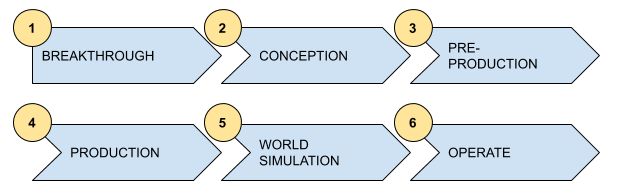
\includegraphics[width=14cm]{10_img/production_stages.png} 
    \caption{Étapes de création d'un jeu vidéo.}
    \label{fig.etapes}
\end{figure}

Les étapes de développement d'un jeu vidéo ne sont pas immuables et dépendent de l'entreprise, du domaine d'activité ou des collaborateurs impliqués dans le projet. La figure \ref{fig.etapes} présente une liste non exhaustive de ces étapes, telle que présentée par Mathieu Nayrolles lors d’un séminaire au LATECE (Laboratoire de recherche sur les Technologies du Commerce Électronique) de l’UQAM, le 10 avril 2019.



\subsection{\emph{Breakthrough}}

Une étape de \emph{Breakthrough} permet de réunir une équipe afin d'effectuer des recherches et des explorations sur des nouvelles mécaniques ou des nouvelles technologies afin de créer du nouveau contenu. Cette étape est optionnelle dans un projet.
Deux exemples :
\begin{itemize}
    \item Une percée technologique, par ex., Google lance Stavia, une plateforme en ligne de jeux vidéos sous forme de catalogue et jouable à 100\% en ligne sans installation en local;
    \item Une percée de Gameplay, par ex., naissance du mode Battle Royale.
\end{itemize}

\subsection{Conception}
%Conception et non concept car c'est là que les documents sont rédigé, on parle non seulement du QUOI mais aussi du COMMENT les documents sont déjà explicites sur le COMMENT le jeu fonctionnera et sera développé

Un document de conception est défini afin d'identifier l'environnement, la faisabilité et l'intérêt commercial du jeu. C'est durant cette étape que les \emph{Game designer} définissent et précisent l'univers, les mécaniques et le déroulement du jeu vidéo en question. Cette étape est majoritairement gérée par les \emph{Game designers} appuyés par les équipes des autres corps de métier. Dans des projets à financements externes, cette étape est cruciale: elle permettra de présenter le projet à un studio avec une première maquette présentant les fondements du jeu.

\subsection{Pré-production}
Durant cette étape, des prototypes sont développés afin de créer une version minimale du jeu. Ces prototypes permettent d'avoir un aperçu jouable des concepts définis durant la phase précédente. 

Un prototype est une coupe verticale de tout le système qui permet de valider ou redéfinir les concepts. Une fois le design bien défini, le prototype plus proche de ce que donnerait le jeu final et la faisabilité du projet confirmée, il est alors possible de rechercher les financements et les ressources nécessaires à la production. Cette étape est gérée par tous les corps de métier dans un studio de développement, tous les aspects du jeu devant être représentés afin de montrer tout le potentiel du prototype.

\subsection{Production}
Une fois les fonds levés et les ressources humaines attitrées au projet, il est alors possible de procéder à la production du jeu vidéo. Tous les corps de métier sont alors représentés et le jeu est développé sous tous ses aspects et dans son intégralité. La plupart du temps le développement est découpé en plusieurs itérations. Chacune d'entre elles permet de vérifier que le jeu respecte bien les concepts définis plus tôt. C'est également à ce moment là que les dernières modifications sont apportées aux concepts afin qu'ils respectent la vision du \emph{Game designer} et génèrent la bonne expérience. Dans le cas o\`u le projet rencontre des contraintes supplémentaires (temps, argent, plateforme, etc.) les concepts peuvent également être revus. Généralement, durant cette étape, le marketing et la publicité autour du jeu commencent à prendre place afin d'informer le public et d'estimer l'impact que peut avoir le jeu.


\subsection{\emph{World Simulation}}
Lors de la \emph{World simulation}, tous les éléments du jeu sont testés et passés au crible. On vérifie que les éléments de jeu sont correctement modélisés, que les sons correspondent bien aux éléments, que les personnages correspondent à ceux décrits dans les documents de conception, etc. Plusieurs questions se posent à ce moment là. 
\begin{itemize}
    \item Est-ce que les éléments interagissent bien entre eux ?
    \item Est-ce que l'univers de jeu est cohérent de bout en bout ?
    \item Est-ce que le \emph{gameplay} est fluide et intuitif ?
    \item Est-ce que l'environnement de jeu est réellement tel que décrit par le \emph{Game designer}?
    \item Est-ce que la bande sonore ou la modélisation graphique génère bien les émotions attendues chez le joueur ?
\end{itemize}


\subsection{\emph{Operate}}
Le jeu est maintenant produit et commercialisé. Une quantité importante de données est ainsi générée. Des bogues peuvent être remontés et corrigés dans des cas de figure particuliers ou inédits non couverts par l'étape de \emph{World simulation}. Des ajustements mineurs peuvent être fais en fonction des besoins ou des demandes des joueurs. Le jeu prend alors toute sa dimension et toute sa vie à travers les joueurs.
Une fois le jeu bien en place et les étapes de corrections et ajustements passées, il est possible alors d'intégrer du nouveau contenu au jeu en repassant par les étapes précédentes. Ce nouveau contenu est généralement intégré au sous forme de mises à jours (gratuites) ou de \gls{dlc} (payantes).



\section{Exploitation et exploration}
\subsection{Exploitation}
Le travail d'exploitation consiste à produire une suite ou un nouveau jeu en utilisant des technologies (moteur, plateformes, etc) ou un \emph{gameplay} déjà existant afin de recréer un jeu ou produire du contenu additionnel. Ceci peut être fait dans un but de fidéliser une clientèle déjà existante en ajoutant du contenu additionnel à un jeu, à offrir une expérience similaire avec des technologie plus récentes (ex : FIFA) ou à offrir une suite à un jeu ayant déjà connu du succès (ex : Dark Souls).

L'exploitation est une part importante du travail d'un studio de développement. De nombreux jeux vidéos récents sont basés sur de l'exploitation de jeux précédents, autant au niveau du \emph{gameplay} qu'au niveau des concepts fondamentaux de jeux précédents. C'est le cas de grosses productions de franchises comme les jeux de EA sports (FIFA, NHL, NBA Live, Madden), les jeux d'action \emph{role-play} de FromSoftware (série des Dark Souls), les jeux d'action aventure de Rockstar (série des GTA) ou les jeux de simulation de Maxi/EA Games (série les Sims). 

\subsection{Exploration}
L'exploration, ou l'innovation, dans le monde du jeux vidéos est essentielle au développement de nouveaux concepts de \emph{gameplay} mais également au développement de nouvelles technologies. La nouveauté est un enjeu essentiel afin d'attirer toujours plus de joueurs. L'investissement dans l'exploration est donc très important pour un studio de développement. De la recherche de nouveaux concepts de jeux, de nouveaux types de \emph{gameplay}, de nouvelles technologies à intégrer ou de la création de nouveaux moteurs de jeux, l'exploration est devenue un facteur essentiel au domaine du jeu vidéo et à son expansion.


\subsection{L'équilibre entre exploitation et exploration}
Dans leur article, Parmentier et al \cite{ParmentierGuy2009Iecd} explorent la capacité des studios à concilier ces deux activités. Ils présentent les enjeux de chacune d'entre elles et leur importance dans le domaine.

Il est nécessaire pour les studios de développement de jeux vidéos de trouver le bon équilibre entre exploitation et exploration. L'exploitation est le développement d'un jeu sur des mécanismes déjà existants où les règles sont déjà établies par un autre jeu ou un opus précédent. L'exploration est la découverte de nouvelles mécaniques de gameplay ou la création de nouveaux outils de développement de jeux (comme un moteur de jeu). Le but est d'offrir aux clients des articles de qualité et attractifs. Cet équilibre est précaire et il est difficile pour un studio de développement d'investir sur les deux domaines à la fois. 



\section{Les moteurs de jeux}
Un moteur de jeu (\emph{Game engine}) est, typiquement, une suite logicielle contenant un framework de mécaniques de jeu permettant d'accélérer le développement d'un jeu vidéo. Il peut inclure une ou plusieures facettes du développement du jeu allant de la physique, aux graphismes, aux sons, aux calculs, à la gestion des périphériques d'entrée/sortie jusqu'à la gestion automatique de l'intelligence artificielle. Voici une liste de certains des moteurs de jeu les plus connus accompagnés des jeux qui en font usage : 
\begin{itemize}
    \item \emph{Unreal Engine} \cite{UnrealEngine} développé par Epic Games : Fortnite, Outlast 2, Dragon Ball Fighter Z, Days Gone.
    \item \emph{Unity Engine} \cite{UnityEngine} développé par Unity Technologies : 7 Days to Die, Cuphead, Ori and the Blind Forest, Pokemon Go.
    \item \emph{CryEngine} \cite{CryEngine} développé par Crytek : Far Cry, Crysis 3, Deceit, Mavericks.
    \item \emph{Frostbite} \cite{FrostbiteEngine} développé par Dice (EA) : Battlefield V, Anthem, FIFA, Need for Speed.
\end{itemize}

Chaque moteur de jeu présente des avantages et des inconvénients en fonction du type de jeu que l'on souhaite développer. Certains moteurs sont axés sur un type de jeu ou une plateforme en particulier afin d'être plus efficaces. 
L'innovation dans les moteurs de jeu est aussi essentielle au développement de nouveaux jeux vidéos. 
Par exemple, un moteur de jeu plus récent pourra intégrer des éléments plus récents comme des graphismes plus réalistes ou détaillés, ou des intelligences artificielles plus évoluées.

\section{Les types de \emph{Gameplay}}
L'exploration peut également consister en la création d'un nouveau mécanisme de \emph{gameplay}. Ce genre d'innovation est plus facilement repérable par les joueurs et plus marquante en ce qui a trait \`a l'expérience de jeu. 

Voici une liste non exhaustive des principaux types de \emph{gameplay} présents dans les jeux vidéos :
\begin{itemize}
    \item MMORPG (\emph{Massive Multiplayer Online Role-Playing Games}) : jeu massivement multijoueur en ligne mettant en scène un jeu de rôle avec différents objectifs à remplir : \emph{leveling}, histoire principale vs.\ secondaire, développement social pour atteindre ces objectifs sous forme de guilde, etc. (ex. : World of WarCraft, Black Desert Online).
    \item \emph{Survival} : le joueur doit survivre aux événements présents dans le jeu. Il peut devoir subvenir à des besoins vitaux, construire de nouveau objets, ou survivre aux autres joueurs présents (ex. : Rust, Ark).
    \item Plateformes : un joueur contrôle un personnage qui se déplace dans un environnement de plateformes et doit avancer tout au long du niveau pour le compl\'eter (ex. : Mario, Donkey Kong).
    \item Simulation de vie : le joueur simule un environnement de vie plus ou moins réaliste en fonction des objectifs du jeu. La simulation peut s'appliquer à un personnage ou à une ville entière. (ex. : Les Sims, SimCity).
    \item FPS (\emph{First Person Shooter}) : le joueur, seul ou en équipe, doit battre des ennemis (IA ou autres joueurs) à l'aide d'armes et d'équipements de combat (ex. : Call of Duty, Halo).
    \item \emph{Beat-em up} : le joueur fait face à des vagues d'ennemis toujours plus fortes (ex. : Bayonnetta, God of War).
    \item RTS (\emph{Real Time Strategy}) : des joueurs se font face dans un jeu o\`u la gestion d'économie, de troupes et de population est omniprésente afin de battre les autres (Age of Empire, Starcraft).
    \item 4X (\emph{eXplore, eXpand, eXploit, and eXterminate}) : proche du RTS, ce type de \emph{gameplay} se base sur une gestion pointue de ressources et de populations afin de pouvoir battre les autres joueurs sous différents aspects et avec différents objectifs de victoire (population maximale, évolution de la société, critères fininanciers, etc.) (ex. : Civilization, Stellaris).
    \item MOBA (\emph{Multiplayer Online Battle Arena}) : c'est un type de \emph{gameplay} o\`u le jeu d'action rencontre le RTS. Plusieurs équipes de joueurs sont téléportées sur un territoire, chaque joueur contrôle un personnage et les joueurs doivent détruire la base de l'équipe adverse (ex. : League of Legends, DOTA).
    \item \emph{Battle Royal} : plusieurs dizaines de joueurs sont parachutés sur un territoire o\`u ils trouvent des armes et doivent s'entretuer~; le dernier survivant est déclaré vainqueur (ex. : Fortnite, PUBG).
\end{itemize}

Les types de \emph{gameplay} évoluent beaucoup. De nouveaux \emph{gameplay}s apparaissent grâce aux recherches exploratoires. Certains modes de jeux à succès deviennent des catégories à part entière. Il est possible de combiner plusieurs modes de jeu afin de créer une nouvelle expérience. Ces divers types de \emph{gameplay} sont classifiés en fonction du type de monde, des objectifs de jeu, des actions nécessaires, etc. Haitz et Law~\cite{HeintzStephanie2015TGGM} ont mis en place une cartographie des genres afin de classifier les différents types de jeux en se basant sur des caractéristiques précises des jeux et de leur \emph{gameplay}. Cependant, il est difficile d'arriver à classifier tous les jeux tellement les genres sont nombreux et entrecoupés. C'est pour cela que la plupart des jeux sont classifiés dans des catégories larges et sont ensuite différenciés par leurs diverses caractéristiques.



\section{Objectif de notre travail de recherche}

\GT{On reverra cette section ultérieurement. Une partie de cela
devrait \^etre dans l'introduction.}

De nombreux défis entourent le développement de jeux vidéos et les outils et méthodes pour y parvenir sont déjà nombreux. Cependant, il devient de plus en plus important de chercher des méthodes afin d'accélérer le développement, sans pour autant impacter la qualité du contenu final. Un \emph{Game designer} se doit d'être précis et concis dans ses descriptions et ses communications afin de communiquer un maximum d'informations et de pouvoir dédier plus de temps à l'exploration, à la recherche artistique et au développement d'un prototype. 



%quoi
Dans ce mémoire, nous allons présenter \gls{gg}, un profil UML \cite{ReferenceBibliographique} qui permet d'outiller le processus de pré-conception d'un jeu vidéo, facilitant ainsi la documentation et la rédaction des documents descriptifs du jeu vidéo en cours d'élaboration.

%rapidité
Destiné à être utilisé dans les premières phases du développement, \emph{Breaktrough} et Pré-conception, ce profil UML permet l'accélération de la documentation à travers un outil visuel représentant les mécaniques et les objets du jeu. Ceci permet de produire un prototype jouable plus rapidement.

%cohérence
L'utilisation d'un profil UML permet d'apporter une structure précise et un cadre de travail rigoureux lors de la conception afin d'assurer la cohérence des modèles durant toute leur durée de vie.

%maintenance & modifications
Lors de sa conception, un jeu vidéo est destiné à évoluer rapidement et sa documentation se verra modifiée de nombreuses fois afin de toujours être la plus pertinente possible. UML permet d'apporter un support visuel à cette documentation mais permet également de rendre les modifications plus faciles en accédant aux objets concernés rapidement et efficacement. 

%pérennité
Effectuer des \emph{mind mapping} est un moyen simple et efficace permettant d'illustrer des idées de manière visuelle. Cependant, le manque de rigueur (modifications erratiques, contenu des données incohérents, manque de structure) et les supports utilisés (feuille de papier ou tableau) lors d'un travail de \emph{mind mapping} n'assure pas du tout la pérennité des informations stockées. Il est en effet compliqué de modifier une photographie d'un \emph{mind map} lors d'une réunion ayant pris place plusieurs semaines auparavant. De par sa structure imposée et précise le standard UML permet de structurer les données, de les stocker sous un format précis et de les maintenir facilement en communiquant sur les modifications effectuées. Ceci permet un stockage beaucoup plus pérenne des informations contenues dans le modèle.

%réutilisation
UML étant un langage de modélisation largement utilisé et approuvé dans le domaine informatique, il est possible d'utiliser de nombreux outils d\'ej\`a existants, d'assurer son intégration et sa réutilisation dans différents cadres et sous différentes formes.

%gdd
Un modèle UML pourra également servir de support à la rédaction d'un \gls{gdd} en organisant les mécaniques de jeu sous forme de catégories réutilisables. Le GDD est la \guillemotleft bible du design \guillemotright \cite{GD_foundations_pedersen} du jeu. Il permet de définir tout le contenu du jeu et toutes les informations nécessaires à son développement sur toute sa durée de vie. 

%generation de code
UML étant reconnu comme un langage de modélisation de logiciels, il peut également être possible d'utiliser les modèles créés en pré-conception afin de faciliter le développement informatique du jeu vidéo. Le modèle peut permettre de créer une structure de projet ou du pseudo code pouvant servir de squelette en début de développement.


